\documentclass[11pt,a4paper]{article}

% Core Packages
\usepackage[utf8]{inputenc}
\usepackage[margin=1in]{geometry}
\usepackage{helvet}
\usepackage{microtype}
\usepackage{booktabs}
\usepackage{tabularx}
\usepackage{amsmath}
\usepackage{enumitem}
\usepackage{hyperref}
\usepackage{xcolor}
\usepackage{pgfplots}
\pgfplotsset{compat=1.17}
\usepackage{caption}

\hypersetup{
    colorlinks=true,
    linkcolor=black,
    urlcolor=blue,
    citecolor=black
}

\renewcommand{\familydefault}{\sfdefault}

\setlist[itemize]{noitemsep, topsep=2pt}
\setlist[enumerate]{noitemsep, topsep=2pt}

\definecolor{tlblue}{HTML}{2C5F8A}
\definecolor{tlgreen}{HTML}{3D8B5F}
\definecolor{tlgray}{HTML}{6B6B6B}

% Title Information
\title{\textbf{\Large TimeLens AI}\\[0.3em]
\large Adaptive Task-Duration Planner: Technical Report on the Minimum Viable Prototype}
\author{
    \textbf{Vansh Jain} (1024030770) \quad
    \textbf{Devyang} (1024030765) \quad
    \textbf{Bhavik} (1024030772)\\[0.5em]
    \small Department of Computer Engineering\\
    \small Thapar Institute of Engineering and Technology
}
\date{September 2026}

\begin{document}

\maketitle
\hrule
\vspace{1.5em}

\begin{abstract}
\noindent TimeLens AI is a local, single-user proof of concept that corrects a person's task-duration
estimates using their own completion history, lays out a deterministic daily timeline from those
corrected durations, and re-sequences remaining work when a task runs late. Rather than a trained
machine-learning model, the prototype uses a transparent statistical baseline: a blended category
bias, a time-of-day multiplier, and an interruption overhead term, so that every prediction can be
explained to the user in plain language. This report documents the implemented system: its
architecture, prediction formula, scheduling rules, data model, demonstration workflow, evaluation
figures observed from the seeded demo, and known limitations, and outlines the scope for a
production-grade extension.
\end{abstract}

\section{Overview}
Task planners typically treat a user's self-reported duration estimate as ground truth and build a
schedule directly from it. In practice, people are systematically biased estimators: some categories
of work reliably run long, performance varies with time of day, and interruptions add overhead that is
rarely budgeted for. TimeLens AI targets this gap at prototype scale: it is a single Next.js
application, with no authentication, cloud service, or external API, that demonstrates the complete
loop of \emph{predict $\rightarrow$ schedule $\rightarrow$ adapt $\rightarrow$ learn} using a local
SQLite database.

\section{Problem Statement}
Conventional task managers function as passive storage systems for user-supplied durations. This
produces four recurring failure modes that the prototype is designed to illustrate:
\begin{itemize}
    \item \textbf{Unmitigated estimation bias.} Users under- or over-estimate durations in
    category-specific, measurable ways, and planners never correct for it.
    \item \textbf{Assumed uniform productivity.} Output varies with time of day, yet planners treat
    every hour as equally productive.
    \item \textbf{Uncaptured interruption cost.} Context switches and interruptions add real overhead
    that is absent from the original estimate.
    \item \textbf{Static schedule degradation.} Once a task overruns, the remainder of the day is left
    unchanged, compounding the delay.
\end{itemize}
TimeLens AI addresses these with an explainable statistical correction rather than a black-box model,
prioritizing transparency and demonstrability over predictive sophistication at this stage.

\section{System Architecture}
The prototype runs as a single Next.js (App Router) application; there is no separate backend, external
API, authentication layer, or cloud dependency.

\begin{itemize}
    \item \textbf{\texttt{src/app}}: server-rendered dashboard and server actions.
    \item \textbf{\texttt{src/components}}: interactive dashboard components.
    \item \textbf{\texttt{src/lib}}: Prisma client, prediction logic, scheduling logic, analytics,
    and seed fixtures.
    \item \textbf{\texttt{src/types}}: framework-independent planning types.
    \item \textbf{\texttt{prisma}}: SQLite schema and seed entry point.
    \item \textbf{\texttt{tests}}: focused Vitest calculation tests.
\end{itemize}

The browser invokes Next.js server actions to perform mutations; those actions call Prisma directly and
revalidate the dashboard. There is no client-side API layer to secure or version, which keeps the
prototype's surface area small while still exercising the full predict-schedule-adapt loop end to end.

\subsection{Technology Stack}
\begin{center}
\begin{tabular}{ll}
\toprule
\textbf{Layer} & \textbf{Technology} \\
\midrule
Application framework & Next.js (App Router), TypeScript \\
Data access & Prisma ORM \\
Persistence & SQLite (local file) \\
Testing & Vitest \\
\bottomrule
\end{tabular}
\end{center}

\section{Prediction Model}
Each new task's duration is corrected using completed \texttt{TaskHistory} records from the same
category:
\begin{equation}
\text{prediction} = \text{estimate} \times \text{category bias} \times \text{time-of-day factor} +
\text{interruption overhead}
\end{equation}

\begin{itemize}
    \item \textbf{Category bias} is the median ratio of actual to estimated duration for that category,
    blended toward a default of $1.10$ until at least six matching records exist.
    \item \textbf{Time-of-day factor} is $0.95$ for morning, $1.15$ for afternoon, and $1.05$ for
    evening tasks.
    \item \textbf{Interruption overhead} adds three minutes per average historical interruption for the
    category, capped at fifteen minutes.
    \item The result is rounded and constrained to a practical range. Confidence is reported as LOW,
    MEDIUM, or HIGH, rising as matching history accumulates.
\end{itemize}

\subsection{Worked Example}
The seeded \emph{Technical Report} history carries a category bias of $1.25$ and an average of three
interruptions. A $60$-minute task scheduled for a $2$:$00$~PM preferred start is therefore corrected as:
\begin{equation}
60 \times 1.25 \times 1.15 + 9 = 95.25 \approx 95 \text{ minutes}
\end{equation}

Figure~\ref{fig:factors} shows the two multiplicative factors that drive this correction across the
categories and times of day used in the seeded demo data.

\begin{figure}[htbp]
\centering
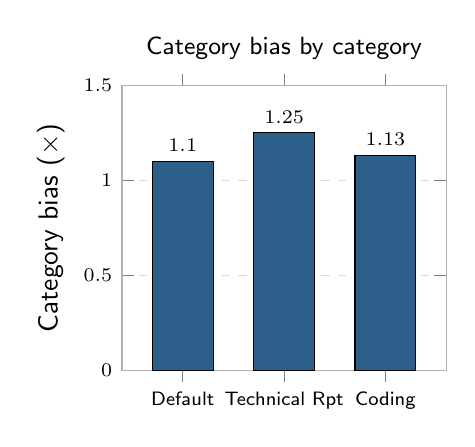
\begin{tikzpicture}
\begin{axis}[
    ybar, bar width=22pt,
    width=0.47\textwidth, height=5.2cm,
    ymin=0, ymax=1.5,
    symbolic x coords={Default,Technical Rpt,Coding},
    xtick=data,
    ylabel={Category bias ($\times$)},
    nodes near coords,
    every node near coord/.append style={font=\scriptsize},
    ymajorgrids, major grid style={dashed,gray!30},
    axis line style={gray!60},
    enlarge x limits=0.3,
    title={\small Category bias by category},
    tick label style={font=\scriptsize}
]
\addplot[fill=tlblue] coordinates {(Default,1.10) (Technical Rpt,1.25) (Coding,1.13)};
\end{axis}
\end{tikzpicture}
\hfill
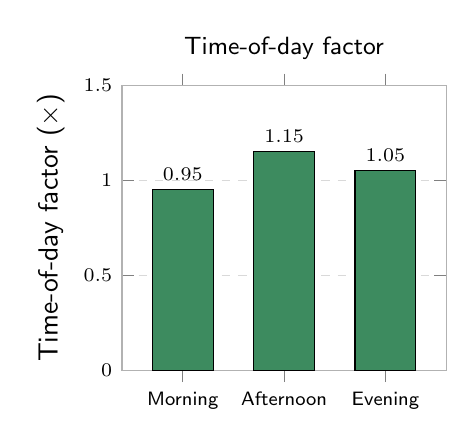
\begin{tikzpicture}
\begin{axis}[
    ybar, bar width=22pt,
    width=0.47\textwidth, height=5.2cm,
    ymin=0, ymax=1.5,
    symbolic x coords={Morning,Afternoon,Evening},
    xtick=data,
    ylabel={Time-of-day factor ($\times$)},
    nodes near coords,
    every node near coord/.append style={font=\scriptsize},
    ymajorgrids, major grid style={dashed,gray!30},
    axis line style={gray!60},
    enlarge x limits=0.3,
    title={\small Time-of-day factor},
    tick label style={font=\scriptsize}
]
\addplot[fill=tlgreen] coordinates {(Morning,0.95) (Afternoon,1.15) (Evening,1.05)};
\end{axis}
\end{tikzpicture}
\caption{Multiplicative correction factors used in the prediction formula, drawn from the seeded demo
data (Technical Report and Coding categories) and the fixed morning/afternoon/evening multipliers.}
\label{fig:factors}
\end{figure}

\section{Scheduling Engine}
Once a duration is predicted, the task is placed into a deterministic daily timeline:
\begin{itemize}
    \item Completed tasks are frozen; their saved schedule fields are never modified.
    \item Pending tasks are ordered by deadline, with priority breaking ties within a two-hour window.
    \item The plan begins at 9:00~AM and runs tasks sequentially using predicted (not estimated)
    minutes.
    \item A task is flagged \emph{at risk} if its scheduled end falls after its deadline.
\end{itemize}

\subsection{Delay Simulation}
The prototype can simulate a fixed $35$-minute delay on any task. This shifts that task's end time and
propagates the same $35$-minute shift to every later pending task, demonstrating adaptive
re-sequencing rather than a static, one-shot plan.

\section{Data Model}
The local SQLite database contains exactly two application models.

\begin{center}
\begin{tabularx}{\textwidth}{>{\bfseries}l X}
\toprule
\textbf{Model} & \textbf{Purpose} \\
\midrule
Task & Current title, category, estimate, prediction, priority, deadline, schedule, status, actual
duration, interruption count, and timestamps. \\
TaskHistory & Immutable completion snapshots used for future predictions and analytics. \\
\bottomrule
\end{tabularx}
\end{center}

Priority is one of \texttt{LOW}, \texttt{MEDIUM}, or \texttt{HIGH}; task status is \texttt{PENDING} or
\texttt{COMPLETED}.

\section{MVP Feature Set}
\begin{itemize}
    \item Create, delete, and complete tasks without authentication or a separate backend.
    \item Store task data and completion history in local SQLite through Prisma.
    \item Explain each predicted duration with category, time-of-day, and interruption factor cards.
    \item Build a deterministic plan from 9:00~AM using deadline, priority, and predicted duration.
    \item Simulate a 35-minute delay and shift the delayed task plus every later pending task.
    \item Record actual duration on completion and update the lightweight analytics panel.
    \item Restore consistent demonstration data on demand with \emph{Reset demo}.
\end{itemize}

\section{Demonstration Workflow}
The recorded demonstration follows a fixed six-step sequence:
\begin{enumerate}
    \item Open the seeded dashboard and point out the four planned tasks and the learning panel.
    \item Enter \emph{Technical Report}, a 60-minute estimate, a 3:00~PM deadline, and an afternoon
    preferred start (the form defaults to 2:00~PM).
    \item Add the task and show its 95-minute predicted duration together with its factor cards and
    explanation.
    \item Inspect its placement in the daily timeline, built from corrected rather than raw durations.
    \item Apply a $+35$-minute delay to the new report and confirm every later pending task shifts by
    35 minutes.
    \item Enter an actual duration, mark the task complete, and observe the completed-task count and
    analytics panel update. Use \emph{Reset demo} to repeat from the original state.
\end{enumerate}

\section{Evaluation and Observed Metrics}
Because the prototype uses an explainable baseline rather than a trained model, evaluation focuses on
\emph{workload correction} and \emph{historical accuracy} rather than classical ML validation metrics.
The figures below are those surfaced live on the seeded demo dashboard.

\begin{center}
\begin{tabular}{lc}
\toprule
\textbf{Dashboard metric} & \textbf{Seeded demo value} \\
\midrule
Pending tasks & 4 \\
Original estimate (sum) & 235 min \\
Predicted workload (sum) & 284 min \\
Extra time detected & +49 min \\
Mean absolute error (completed tasks) & 13 min \\
Completed tasks recorded & 12 \\
\bottomrule
\end{tabular}
\end{center}

\begin{figure}[htbp]
\centering
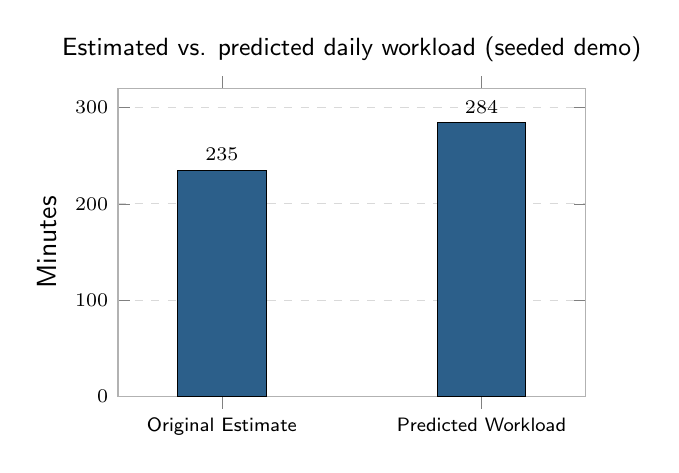
\begin{tikzpicture}
\begin{axis}[
    ybar, bar width=32pt,
    width=0.62\textwidth, height=5.5cm,
    ymin=0, ymax=320,
    symbolic x coords={Original Estimate,Predicted Workload},
    xtick=data,
    ylabel={Minutes},
    nodes near coords,
    every node near coord/.append style={font=\scriptsize},
    ymajorgrids, major grid style={dashed,gray!30},
    axis line style={gray!60},
    enlarge x limits=0.4,
    title={\small Estimated vs. predicted daily workload (seeded demo)},
    tick label style={font=\scriptsize}
]
\addplot[fill=tlblue] coordinates {(Original Estimate,235) (Predicted Workload,284)};
\end{axis}
\end{tikzpicture}
\caption{TimeLens AI's correction adds 49 minutes of previously unbudgeted time across the four
pending demo tasks, surfacing the gap between what users estimate and what the historical model
predicts.}
\label{fig:workload}
\end{figure}

The mean absolute error of 13 minutes across 12 completed tasks is reported directly by the analytics
panel and reflects the gap between each task's predicted and actual duration under the current
category-bias and time-of-day model; it is a descriptive statistic over the seeded history rather than
a held-out test-set metric, since the MVP does not yet separate training and evaluation data.

\section{Known Limitations}
\begin{itemize}
    \item The planner builds a single sequential day and does not model breaks, calendars,
    working-hour limits, dependencies, or recurring tasks.
    \item The prediction is deliberately a transparent statistical baseline; there is no model training
    or personalization across multiple users.
    \item Preferred start is used only for the initial time-of-day prediction; it is not a persisted
    scheduling constraint, since the MVP schema is intentionally minimal.
\end{itemize}

\section{Phase 2 / Production Roadmap}
\begin{itemize}
    \item Multiple planning days, availability windows, and task dependencies.
    \item More detailed interruption capture and trend visualizations.
    \item A user-controlled calibration view and richer model evaluation.
    \item Optional export and calendar integrations, while keeping the core planner understandable.
    \item Longer term: accounts, cloud persistence, gradient-boosted or other trained ML models, and
    notification delivery.
\end{itemize}

\section{Setup and Reproduction}
\begin{enumerate}
    \item Requires Node.js 20 or later.
    \item \texttt{npm install}
    \item \texttt{npm run setup}: generates the Prisma client, creates/updates the SQLite database,
    and loads fresh demo data.
    \item \texttt{npm run dev}: then open \url{http://localhost:3000}.
    \item \texttt{npm test}: runs the Vitest calculation checks.
\end{enumerate}
To recreate the recorded demonstration while the local server is running: \texttt{npm run
demo:record}, then \texttt{npm run demo:mp4}, then \texttt{npm run db:seed} to restore the original
demo state.

\section{Summary}
TimeLens AI's MVP demonstrates, in a single local codebase, that a fully explainable statistical
correction (category bias, time-of-day adjustment, and interruption overhead) is enough to show
a complete predict-schedule-adapt-learn loop without authentication, cloud infrastructure, or a trained
model. The seeded demo's own figures (a 13-minute mean absolute error over 12 completed tasks and a
49-minute workload correction across four pending tasks) provide concrete, reproducible evidence for
the core idea, while the documented limitations set clear boundaries for what remains prototype-only
versus what a production system would need to add.

\end{document}
